\chapter{{Data Synchronization}}%
\label{ch:synchronisation}
% nestjs, mysql, accounts


\section{{Backend}}%
\label{sec:backend}
The best solution to implement back-end is to choose framework supporting same language as we used in front-end application. It gives an opportunity to share code and librarie between clients and server app.

\begin{displayquote}
    NestJS is a framework for building scalable Node.js server-side applications uses progressive JavaScript,  fully supports TypeScript (still enables developers to code in pure JavaScript) and combines elements of OOP (Object Oriented Programming) \autocite{NyakundiOOP}. Under the hood, Nest makes use of robust HTTP Server frameworks like ExpressJS \autocite{ExpressJS}. 
    Nest provides a level of abstraction above these common Node.js frameworks (Express/Fastify), but also exposes their APIs directly to the developer. This gives developers the freedom to use the myriad of third-party modules which are available for the underlying platform \autocite{NestJsDoc}.
\end{displayquote}

Following NestJs documentation Nest CLI will be installed with command:
\begin{verbatim}
    npm i -g @nestjs/cli
\end{verbatim}

Next, new project (in this case 'server' is the project name) will be scaffold with CLI command:
\begin{verbatim}
    nest new server
\end{verbatim}



\section{{Database}}%
\label{sec:database}

To store data on the server for this project the MySQL database is used \autocite{MySQL}. It's one of the most popular open-source relational database management system.

First we need to create a new database, new user and update privileges in local development environment

\begin{listing}[H]
    \begin{minted}{sql}
    CREATE DATABASE medikoproof;
    CREATE USER medikohogent@localhost IDENTIFIED BY '*PASSWORD*';
    GRANT ALL PRIVILEGES ON medikoproof.* TO 'medikohogent'@'localhost';
    FLUSH PRIVILEGES;
    \end{minted}
\caption[SQL command to setup database and add user]{SQL command to setup database and add user.}
\end{listing}


To map the JavaScript objects into relational database tables we need an object-relational mapping system (ORM) \autocite{AmblerORM}. For integrating with SQL, NestJS provides a package for TypeORM \autocite{TypeORM}, according to the documentation - one of the most mature Object Relational Mapper (ORM) available for TypeScript and because it's written in TypeScript, it integrates well with the Nest framework \autocite{NestJsDoc}. 

The required packages are added with the following commands:

\begin{verbatim}
    npm install --save @nestjs/typeorm typeorm mysql2
\end{verbatim}

To improve migrations, additional scripts have been added to the package.json file.

\begin{listing}[H]
    \begin{minted}{json}
"typeorm:prepare": "npm run build && npx typeorm -d dist/db/config/data-source.js",
"migration:log": "npm run typeorm:prepare -- schema:log",
"migration:generate": "npm run typeorm:prepare -- migration:generate -p",
"migration:create": "npx typeorm migration:create",
"migration:run": "npm run typeorm:prepare -- migration:run",
"migration:revert": "npm run typeorm:prepare -- migration:revert"
    \end{minted}
\caption[Migrations scripts]{Additional migrations scripts added to the package.json}
\end{listing}


New module is created with a NestJs CLI command which automatically adds folders and files:

\begin{verbatim}
    nest generate resource modules/users

    modules
    └── users
        ├── entities
        │   └── user.entity.ts
        ├── users.module.ts
        ├── users.service.spec.ts
        └── users.service.ts
\end{verbatim}


Now, we need to create new table with users in the database. To achieve that a migration script is created and executed with the following commands:

\begin{verbatim}
    npm run migration:generate -- db/migrations/user
    npm run migrations:run
\end{verbatim}

\begin{listing}[H]
\begin{minted}{sql}
CREATE TABLE `user` (
    `id` int NOT NULL AUTO_INCREMENT,
    `name` varchar(255) NOT NULL,
    `password` varchar(255) NOT NULL,
    `created_at` datetime(6) NOT NULL DEFAULT CURRENT_TIMESTAMP(6),
    `updated_at` datetime(6) NOT NULL DEFAULT CURRENT_TIMESTAMP(6) ON UPDATE CURRENT_TIMESTAMP(6),
    UNIQUE INDEX `IDX_065d4d8f3b5adb4a08841eae3c` (`name`),
    PRIMARY KEY (`id`)
) ENGINE = InnoDB
\end{minted}
\caption[TypeORM SQL migration script]{'Users' repository SQL migration script generated by TypeORM}
\end{listing}




\section{{Authentication}}%
\label{sec:authentication}

Accounts management is an essential part of every software solution using client-server architecture. NestJS framework provides support for Jason Web Token based Authentication (JWT) \autocite{JWT} what is one of the most popular approaches. The package which helps with token manipulation, including generating and verifying can be installed with the following command:

\begin{verbatim}
    npm install --save @nestjs/jwt
\end{verbatim}

A new module 'auth' is added inside 'server' folder with Nest CLI command:
\begin{verbatim}
    nest generate resource modules/auth
\end{verbatim}

The 'auth' module controller provides endpoints for login, register and profile information which is protected by the authorization guard.

\begin{listing}[H]
    \begin{minted}{ts}
    @Controller('auth')
    export class AuthController {
        constructor(private authService: AuthService) {}

        @Public()
        @HttpCode(HttpStatus.OK)
        @Post('login')
        signIn(@Body() dto: LoginDto) {
        return this.authService.login(dto.username, dto.password);
        }

        @Public()
        @HttpCode(HttpStatus.OK)
        @Post('register')
        register(@Body() dto: RegisterDto) {
        return this.authService.register(dto.username, dto.password);
        }

        @UseGuards(AuthGuard)
        @Get('profile')
        getProfile(@Request() req) {
        return req.user;
        }
    }
    \end{minted}
\caption[Authentication Controller in Nest module]{Authentication Controller in the Nest 'auth' module}
\end{listing}


Passwords are hashed with 'bcrypt' library \autocite{bcryptTemoye}.


\begin{figure}[H]
    \centering
    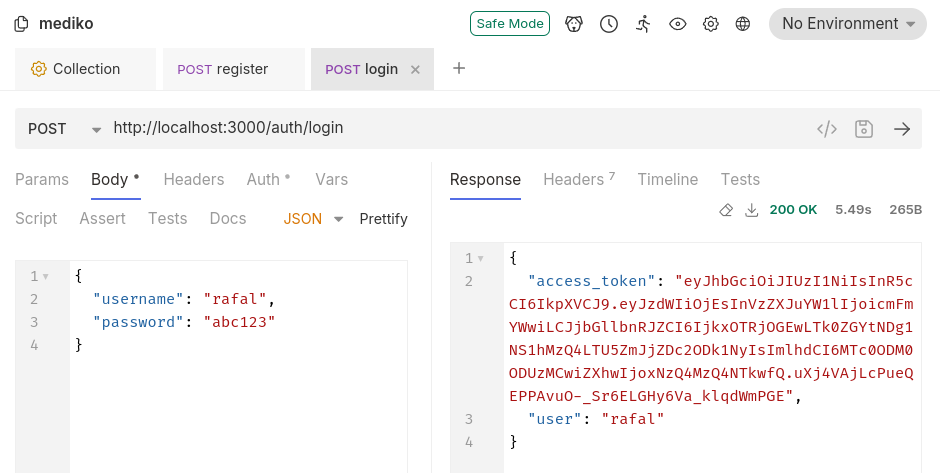
\includegraphics[width=0.8\textwidth]{rest-login.png}
    \caption[Login operation in rest client]{\label{fig:restlogin} Login operation being tested in rest client }
\end{figure}


\section{{Refresh tokens}}%
\label{sec:refreshtoken}

There are two main types of tokens commonly used in web development: access token and refresh token. Access tokens are used to access resources, while refresh tokens are used to get new access tokens when the old ones expire. When an access token expires, a refresh token can be used to get a new one without making the user log in again. Refresh tokens are usually stored securely on the authorization server.

\begin{figure}[H]
    \centering
    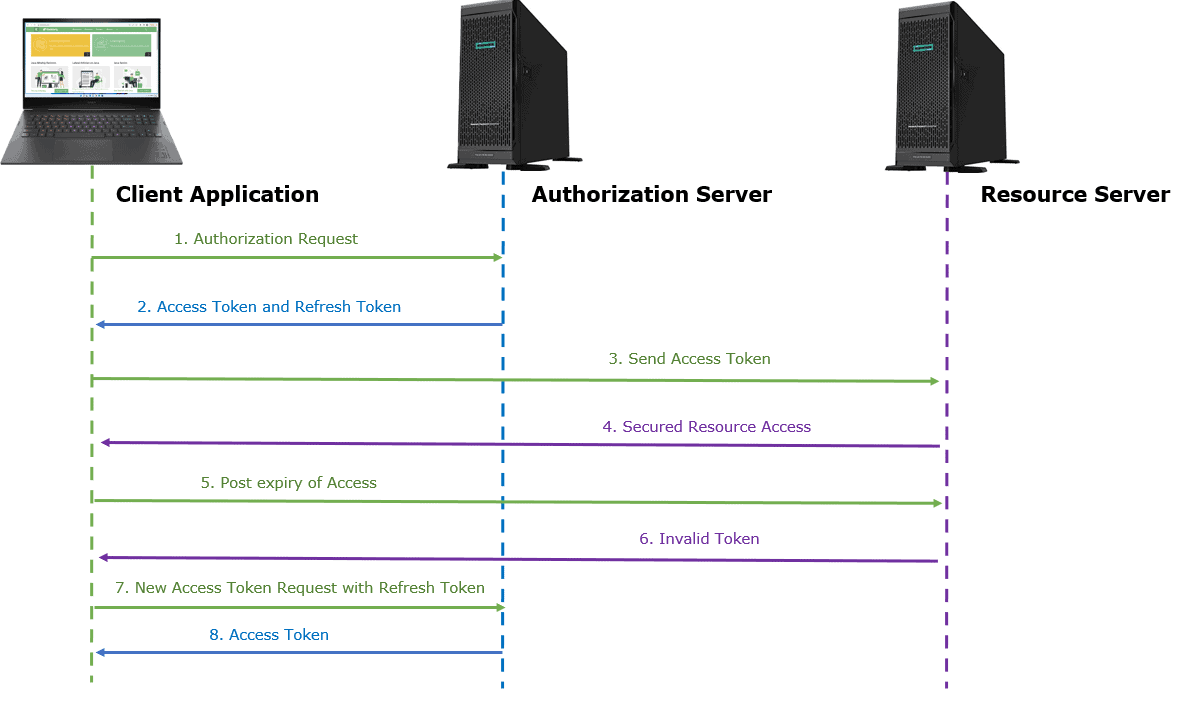
\includegraphics[width=0.8\textwidth]{refresh-token.png}
    \caption[Refresh token authentication strategy diagram ]{\label{fig:refreshtoken} Refresh token authentication strategy diagram \autocite{RoyRefreshToken}. }
\end{figure}

In Authentication controller a new 'refresh' endpoint has been implemented. Refresh tokens will be saved in the database. For this proof-of-concept project Resource-Server and Authorization-Server are integrated.

\begin{figure}[H]
    \centering
    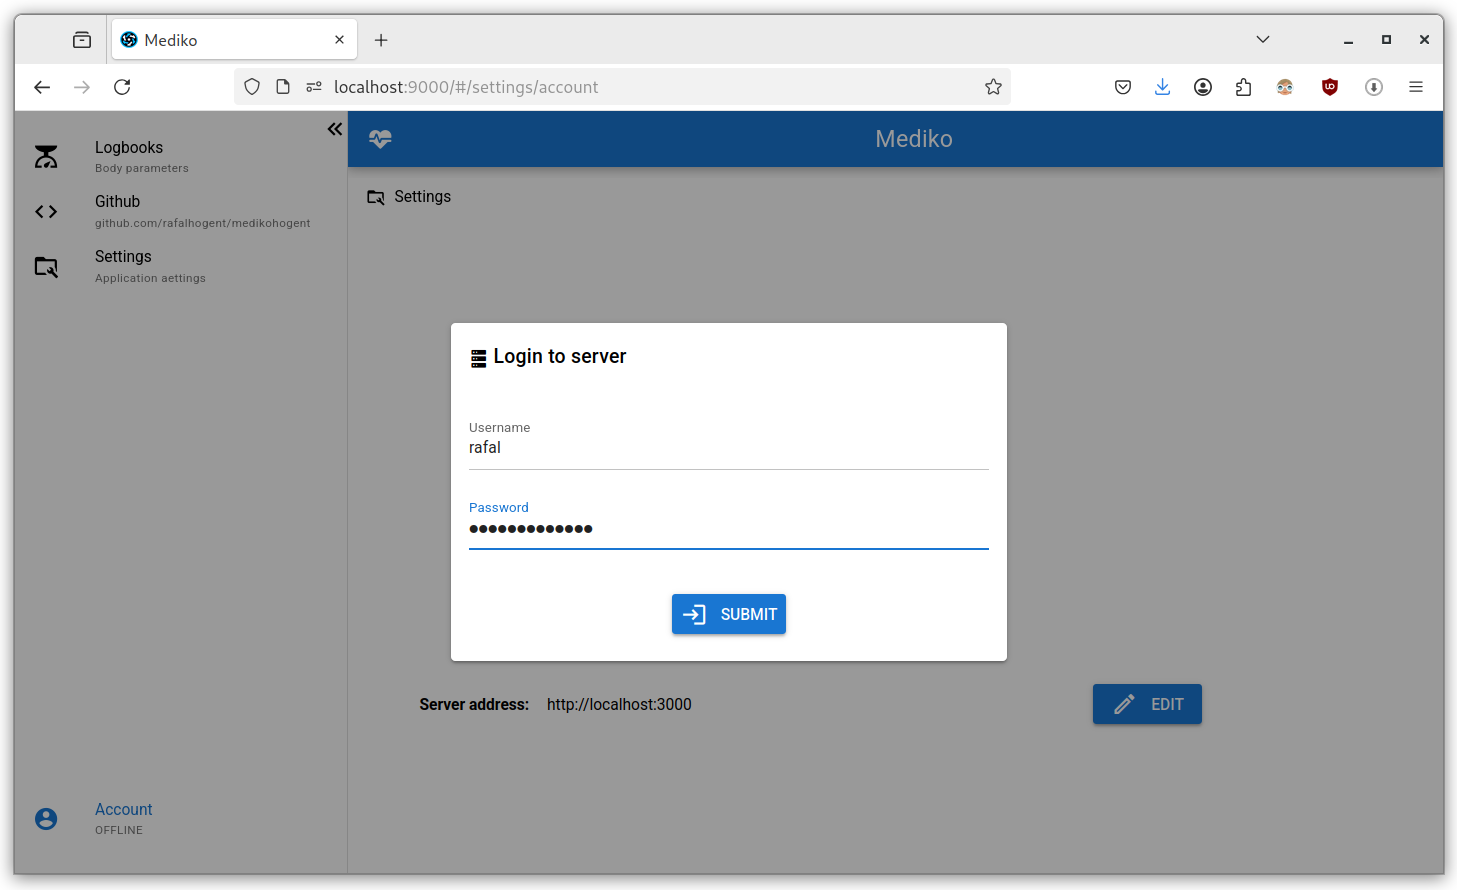
\includegraphics[width=0.7\textwidth]{loginform.png}
    \caption[Proof-of-concept Login form]{\label{fig:loginform} Login Form Implementedin in client application }
\end{figure}


\section{{Synchronization}}%
\label{sec:synchronization}

To let users manage their data in different situations on different devices we need to implement a synchronization strategy. 

Data synchronization refers to the process of ensuring that two or more locations have the same data. In real-time applications, this means that any changes made to the data in one location should be reflected in all other locations sometime almost immediately, sometime with delay. This can be particularly tricky when users are offline or when there are multiple users making changes simultaneously \autocite{SyncPeerDH}.

A simple synchronizing mechanism will be implemented for the purposes of our application, several things need to be considered:
\begin{itemize}
    \item we need not only to let users remove items, but also inform other clients, that this items are deleted. it is possible, that some clients remain inactive for a very long time.
    \item default behavior when authenticated: after registration of new account all local data uploaded to server, after successful login - all local data are cleared local collection is replaced with the newly imported
    \item removed items stay on server, properties are cleared ( = set to null ), isDeleted field is set to TRUE, deletedAt field set to current date-time
\end{itemize}

\begin{figure}[H]
    \centering
    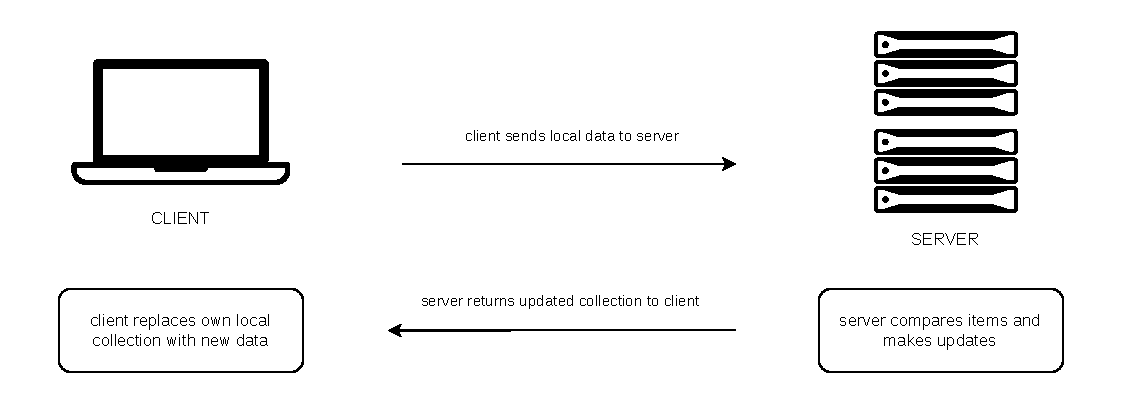
\includegraphics[width=0.8\textwidth]{sync-diagram.eps}
    \caption[Synchronization strategy diagram]{\label{fig:syncdiagram} Diagram illustrating the data synchronization strategy  }
\end{figure}

\begin{listing}[H]
    \begin{minted}{ts}
  async syncLogbooksByUser(syncDto: LogbookSyncDto, userId: number) {
// (...)
  const logsToRemove: Log[] = [];
  clientLogbooks?.forEach(async (clb) => {
    const dblogbook = dbLogbooks.find((dblb) => dblb.id == clb.id);
    if (dblogbook) {
      if (clb.isDeleted && !dblogbook.isDeleted) {
        dblogbook.makeDeleted();
        logsToRemove.push(...dblogbook.logs);
      } else if (!dblogbook.isDeleted) {
        if (
          clb.updatedAt && dblogbook.updatedAt && 
          clb.updatedAt > dblogbook.updatedAt
        ) {
          dblogbook.update(clb);
        }
        clb.logs.forEach((cl) => {
          const dblog = dblogbook.logs.find((l) => l.id == cl.id);
          if (dblog) {
            if (!dblog.isDeleted && cl.isDeleted) {
              dblog.makeDeleted();
            } else if (!dblog.isDeleted) {
              if (
                dblog.updatedAt && cl.updatedAt &&
                dblog.updatedAt < cl.updatedAt
              ) {
                dblog.update(cl as LogDto);
              }
            }
          } else {
            dblogbook.logs.push(cl);
          }
        });
      }
    } else {
      clb.owner = { id: userId } as User;
      dbLogbooks.push(clb);
    }
  });
  const savedLogbooks = await this.logbooksRepo.save(dbLogbooks);
  if (logsToRemove.length) await this.logsRepo.remove(logsToRemove);
  return savedLogbooks;
}
    \end{minted}
\caption[Synchronization implementation]{Synchronization implementation - a part of syncService method in backend application}
\end{listing}


